\section{Estimation} \label{sec:estimation}

\subsection{Naive estimators and their properties in the non informative selection case}
A common approach to achieve a valid variogram estimator is composed by \emph{estimation} and \emph{fitting} of the variogram. In the former, an estimate of the variogram is obtained, while the latter phase is necessary since the estimators used in the first phase are usually not conditionally negative-definite.

Under the assumption of costant-mean, an estimator based on the method of moments is \citep{matheron1962traite}
\begin{equation} \label{eq:variogram_hat}
2\hat{\gamma}\left(h\right)=\frac{1}{|N\left(h\right)|}\sum_{N\left(h\right)}{\left(\Signal\left(\position_{i}\right)-\Signal\left(\position_{j}\right)\right)^{2}},\forall h\in\mathbb{R}^{d}
\end{equation}
where $N\left(h\right)=\lbrace\left(\position_{i},\position_{j}\right):\position_{i}-\position_{j}=h;i,j=1,...,n\rbrace$ and $|N\left(h\right)|$ is the number of distinct pairs in $N\left(h\right)$. 

When data are irregularly spaced in $\mathbb{R}^{d}$, we can use
\begin{equation} \label{eq:variogram_hat1}
2\hat{\gamma}_{s}\left(h\left(l\right)\right)=ave\lbrace\left(\Signal\left(\position_{i}\right)-\Signal\left(\position_{j}\right)\right)^{2}:\left(\position_{i},\position_{j}\right)\in N\left(h\right);h\in T\left(h\left(l\right)\right)\rbrace
\end{equation}
where the region $T\left(h\left(l\right)\right)$ is a specified tolerance region in $\mathbb{R}^{d}$ around $h\left(l\right)$ $l=1,\dots,K$ {\color{red} Check variable $l$}.

A robust version of \eqref{eq:variogram_hat} is given by \citep{cressie1980robust}
\begin{equation} \label{eq:variogram_hat_robust}
2\hat{\gamma}_{r}\left(h\right)=\Bigg\lbrace\frac{1}{|N\left(h\right)|}\sum_{N\left(h\right)}{|\Signal\left(\position_{i}\right)-\Signal\left(\position_{j}\right)|}^{1/2}\Bigg\rbrace ^{4}
/ \left(0.457 + 0.494/|N\left(h\right)|\right)
\end{equation} 
and corresponding smoothed version
\begin{equation}
2\hat{\gamma}_{rs}=\left[med\lbrace|\Signal\left(\position_{i}\right)-\Signal\left(\position_{j}\right)|^{1/2}:\left(\position_{i},\position_{j}\right)\in N\left(h\right);h\in T\left(h\left(l\right)\right)\rbrace\right]^{4}/B\left(h\right)
\end{equation}
where $med$ is the median of the sequence and $B\left(h\right)$ is a correction-term for bias (asymptotically $B\left(h\right)=0.457$).

A non-parametric approach to variogram estimation can be achieved by the use of kernel estimator

\begin{equation}
2\hat{\gamma}\left(h\right)=\frac{\sum_{i}\sum_{j}{w_{ij}\left(h\right)\left(\Signal\left(\position_{i}\right)-\Signal\left(\position_{j}\right)\right)^{2}}}{\sum_{i}\sum_{j}{w_{ij}\left(h\right)}}
\end{equation}
where $w_{ij}=K\left(\frac{h-||\position_{i}-\position_{j}||}{g}\right)$, $K$ is a symmetric, zero-mean (bounded) and $g$ is a positive number called bandwith.

{\color{red}FP: I do not know if the following makes sense.} To sum up, we can write a general estimator form for the \emph{naive estimated variogram}
\begin{equation} \label{eq:g_hat}
    \hat{G}(h)=\sum_{ij\in\Sample}{\beta_{ij}(h)(\Signal(\position_{i})-\Signal(\position_{j}))(\Signal(\position_{i})-Y(\position_{j}))^{T}}
\end{equation}
where the term $\beta_{i,j}$ is a mapping that depends on the particular estimator used (and sample selected).

Once the estimated variogram is obtained (or \emph{empirical}), a model is fitted to it in order to achieve a valid variogram. At this stage, we are searching for a valid variogram ``closest'' to the empirical one, and typically we look into a subset of valid variograms $P=\lbrace2\gamma:2\gamma\left(\cdot\right)=2\gamma\left(\cdot;\theta\right);\theta\in\Theta\rbrace$. The best element of $P$ can be searched through several good-of-fitness criteria. Maximum Likelihood estimator relies heavily on Gaussian assumption, while Least Squares method requires few assumption about $Y\left(\position\right)$.

In particular, with ML we assume that the data $\Signal$ are multivariate Gaussian $(\textbf{X}\boldsymbol{\beta},{\color{red}\provar_{\position,\position^{'};\parampop}}$. The negative loglikelihood is {\color{red} FP: notation needs to be checked.} 
\begin{equation} \label{fit:ML}
L\left(\boldsymbol{\beta},\parampop\right)=\left(n/2\right)\log{\left(2\pi\right)}+\left(1/2\right)\log{|\provar_{\position,\position^{'};\parampop}|}
+\left(1/2\right)\left(\Signal-\textbf{X}\boldsymbol{\beta}\right)^{T}\provar_{\position,\position_{'};\parampop}^{-1}\left(\Signal-\textbf{X}\boldsymbol{\beta}\right)
\end{equation}
with estimators $\boldsymbol{\hat{\beta}}$ and $\hat{\parampop}$ satisfying $L\left(\boldsymbol{\hat{\beta}},\hat{\parampop}\right)=\inf{\lbrace L\left(\beta,\parampop\right):\boldsymbol{\beta}\in\mathbb{R}^{{\color{red}q}},\parampop\in\Theta\rbrace}$.

%REML estimators are obtained by applying maximum likelihood over error contrasts instead of the original data. %In the context of variogram estimation, the idea is to apply the likelihood over $\textbf{W}=\left(\Signal\left(1\right)-\Signal\left(2\right),\Signal\left(2\right)-\Signal\left(3\right),\dots,\Signal\left(n-1\right)-\Signal\left(n\right)\right)$
%Defining a vector of $n-\text{rank}\left(\Position\right)$ linearly independent (error) contrasts as $R=A^{T}\Signal$, where $A$ is an $\left(n-1\right)\times n$ matrix with elements
%\[
%a_{ij}=
%\begin{cases}
%1 &\text{for }i=j,j=1,\dots,n-1, \\
%-1&\text{for }i=j+1,j=1,\dots,n-1,\\
%0 &\text{elsewhere.}
%\end{cases}
%\]
%we have that $R\sim N\left(\textbf{0},A^{T}\provar_{\position,\position^{'};\parampop}A\right)$, which does not depend on $\boldsymbol{\beta}$. Moreover, if $A$ satisfies $AA^{T}=I-\Position\left(\Position^{T}\Position\right)^{-1}\Position^{T}$ and $A^{T}A=I$, we then have the following negative likelihood
%\begin{align*}
%L_{R}\left(\parampop\right)&=\left(\left(n-q\right)/2\right)\log{\left(2\pi\right)}-\left(1/2\right)\log{|\Position^{T}\Position|}+\left(1/2\right)\log{|\provar_{\position,\position^{'};\parampop}|}\\&+\left(1/2\right)\log{|\Position^{T}\provar_{\position,\position^{'};\parampop}^{-1}\Position |}+\left(1/2\right)\Signal^{T}\Pi\left(\parampop\right)\Signal
%\end{align*}
%where $\Pi\left(\parampop\right)=\provar_{\position,\position^{'};\parampop}^{-1}-\provar_{\position,\position^{'};\parampop}^{-1}\Position\left(\Position^{T}\provar_{\position,\position^{'};\parampop}^{-1}\Position\right)^{-1}\Position^{T}\provar_{\position,\position^{'};\parampop}^{-1}$ . Therefore, the REML estimate of $\parampop$ is obtained by minimizing $L_{R}\left(\parampop\right)$ over $\parampop$.

The LS minimizing problem can be written as 
\begin{equation}
min\lbrace\left(2\tilde{\gamma}-2\gamma\left(\theta\right)\right)^{T}W^{-1}\left(\tilde{\gamma}-\gamma\left(\theta\right)\right)
\end{equation}
where $2\tilde{\gamma}$ is the empirical variogram, $2\gamma\left(\theta\right)$ is a valid model variogram with the exact form known except the parameter $\theta$, and $W$ is a weight matrix. If $W$ is an identity matrix, Ordinary Least Square criterion is employed; in case of $W=V$, with $V$ variance-covariance matrix, we have Generalized Least Square criterion, and if $V$ is diagonal, Weighted Least Square criterion is achieved.


Exact finite-sample distribution theory for estimators and corresponding variance estimators are available only in special circumstances (e.g. Jensen 1988). Therefore, simulations or approximation theory need to be employed in order to deal with intractable distribution theory. \cite{zimmerman1991comparison} presented a Monte Carlo comparison of different estimators, when two intrinsically stationary isotropic Gaussian random processes in $\mathbb{R}^{2}$ and various sampling intensities are taken into account. With regard to the MLE, different Authors agree that such approach can suffer from bias. \cite{warnes1987problems} illustrate potential problems by simulations of some simple spatial process, and \cite{mardia1989multimodality} indicate that these problems are caused by likelihoods not twice differentiable in $\parampop$. Moreover, a general conclusion that emerges from a set of several works based on simulations (Haining 1978c, Mardia and Meshall 1984, Swallow and Monahan 1984, Haining et al 1989, Zimmerman and Zimmerman 1991) is that the bias of MLE tends to be negative when the spatial dependence is positive, especially for small sample size. %{\color{red}and asymptotic variances of small-scale variation parameters are good approximation to exact variances only when the spatial dependence is weak.}

For approximation theory, Cressie talks about two type of asymptotic theories {\color{red} pp }. \emph{Infill asympotics} refers to the the possibility to increase the sample size to infinity while the finite domain $D$ is kept fixed, whereas \emph{increase-domain asymptotics} refers to the situation where we take more units by means of increase the domain $D$. 

%Taken as it is from Cressie book (Section 7.3.1): when making inference on a random field $\lbrace Z(s):s\in D\rbrace$ from data $Z=(Z(s_{1},Z(s_{2}),\dots,Z(s_{n}))$, exact distribution theory of estimators, predictors, test statistics, and so on, is rarely available. Asymptotic distribution theory is the natural place to run for approximations, although, spatially, there are number of ways $n$ might tend to infinity.

%The \emph{naive estimated variogram} is 
%\begin{equation} \label{eq:g_hat}
    %\hat{G}(h)=\sum_{ij\in\Sample}{\beta_{ij}(h)(\Signal(\position_{i})-\Signal(\position_{j}))(\Signal(\position_{i})-Y(\position_{j}))^{T}}
%\end{equation}
%In equation \eqref{eq:g_hat}, the term $\beta_{i,j}$ is a mapping that may depend on the sample selected.
%Below we give possible definitions of $\beta_{i,j}$:
%\begin{equation}
    %\beta(\position_1,\position_2,h)=
    %\left|\begin{array}{l}
    %1 \text{ if } |\position_1-\position_2|=h, 0 \text{ otherwise}\\
    %\paramnuisance(\frac{|\position_{i}-\position_{j}|-h}{\alpha})
    %\end{array}\right.
%\end{equation},
%For binned estimation, a finite partition $(B_1,\ldots,B_n)$ of $\mathbb{R}^+$ is given as well as an element $h_k$ of each element $B_k$ of the partition. 
%Then the covariogram is first estimated for each $h_k$, as 
%...
%Then a covariogram is fitted 
%...
%In the following, we will not consider binned estimation.
%where {\color{red} $\paramnuisance$ is ..., and the bins $\mathrm{bin}_h=\left\{(i,j)\in\Sample^2\mid \left|\position_i-\position_j\right|\in [a_h,b_h)\right\}$}

\subsection{Properties of the sample in the general case (including informative)}

\subsection{Naive estimation}
 Naive estimation of the population covariogram:
 $E[naive~Covariogram]\neq$ pop cov,
 $E[naive~Covariogram]=$ sample theoretical cov, 
 with illustrative figures.
{\color{red} I had to move it there. We cannot have this figure without having defined the estimates of the covariogram}
\begin{figure}[H]
\caption{Naive estimation of the semivariogram}
\label{fig:4}
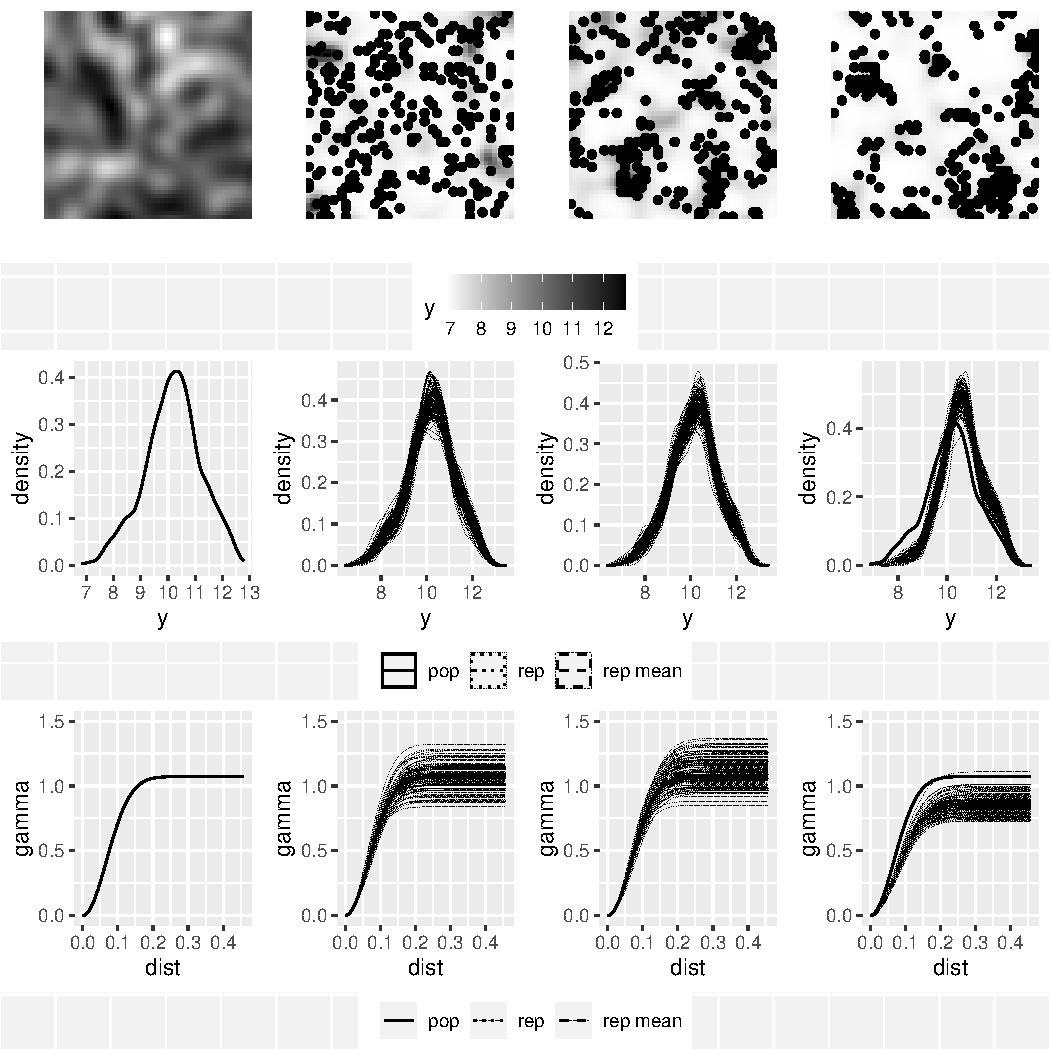
\includegraphics{fig/figure4.pdf}
\end{figure}
